\newpage
% \chapter{Smart Grid in ambiente cloudificato}
\chapter{Il Paradigma Cloud-Native per le Infrastrutture Smart Grid}


Nel capitolo precedente è stata delineata l'architettura fondamentale della Smart Grid descrivendo i componenti tecnologici chiave dei domini del consumatore e operazionale. Questa analisi ha evidenziato come sistemi quali HES, MDMS ed EMS/DMS richiedano un'elevata capacità di calcolo, scalabilità e gestione di enormi volumi di dati. La risposta tecnologica a queste esigenze emergenti risiede nel \textit{Cloud Computing}. Nell'Allegato \ref{allegato:Secondo-allegato}, come approfondimento, vengono presentati i concetti fondamentali e i principali vantaggi in termini di flessibilità, resilienza ed efficienza del \textit{Cloud Computing}.


Questa sezione si propone di esplorare un modello architetturale per una Smart Grid basata su un approccio \textit{Cloud-Native} decentralizzato, analizzando come tale implementazione possa rispondere alle sfide operative della rete moderna e, al contempo, introdurre nuove superfici di attacco e problematiche di sicurezza informatica.

% -------------------------ALLEGATI-----------------------------

% % \chapter{Cloudificazione delle Smart Grid: \\Architettura e Strategie di mitigazione}

% % Nel precedente capitolo ho trattato l'architettura della rete elettrica: Produzione, Trasmissione, Distribuzione ed Utenze Finali, nonché descritto abbastanza nel dettaglio i principali componenti del dominio del consumatore e del dominio operazionale.

% Nel capitolo precedente è stata delineata l'architettura fondamentale della Smart Grid descrivendo i componenti tecnologici chiave dei domini del consumatore e operazionale. Questa analisi ha evidenziato come sistemi quali HES, MDMS ed EMS/DMS richiedano un'elevata capacità di calcolo, scalabilità e gestione di enormi volumi di dati.La risposta tecnologica a queste esigenze emergenti risiede nel Cloud Computing. 


% % In questa sezione, invece, mi occuperò di introdurre il Cloud Computing con i suoi principali vantaggi per poi presentare una possibile implementazione di una Smart Grid in un ambiente \textit{Cloud Native} decentralizzato.



% Questa sezione si propone di esplorare come l'adozione di paradigmi cloud stia trasformando le infrastrutture della rete intelligente. Inizialmente, verranno introdotti i concetti fondamentali del Cloud Computing e i suoi principali vantaggi in termini di flessibilità, resilienza ed efficienza. Successivamente, verrà presentato un modello architetturale per una Smart Grid basata su un approccio \textit{Cloud-Native decentralizzato}, analizzando come tale implementazione possa rispondere alle sfide operative della rete moderna e, al contempo, introdurre nuove superfici di attacco e problematiche di sicurezza informatica.


% \section{Introduzione al Cloud Computing}

% % Da almeno due decenni il nome \textit{Cloud Computing} ha iniziato a diffondersi a profusione, con una crescita significativa data grazie a piattaforme come Amazon Web Service (AWS), Google Cloud Platform (GCP) e Azure la piattaforma cloud di Microsoft.

% Negli ultimi due decenni, il \textit{Cloud Computing} si è affermato come il paradigma dominante per l'erogazione di servizi informatici, una transizione accelerata dalla maturità di piattaforme leader come Amazon Web Services (AWS), Microsoft Azure e Google Cloud Platform (GCP).


% Formalmente, il National Institute of Standards and Technology (NIST) definisce il Cloud Computing come "un modello per abilitare un accesso di rete on-demand, conveniente e ubiquo a un pool condiviso di risorse di calcolo configurabili (es. reti, server, storage, applicazioni e servizi) che possono essere rapidamente approvvigionate e rilasciate con un minimo sforzo di gestione o interazione con il fornitore di servizi" \cite{NIST-cloud-computer}


% % Con il termine \textit{Cloud Computing}, si intende la fruizione di servizi quali: software, informazioni, intere infrastrutture di server ecc., utilizzando internet ("Il Cloud"). Eliminando la necessità per gli individui e le aziende di autogestire le risorse fisiche.
% % e di pagare solo per ciò che utilizzano.

% In termini più semplici, il Cloud Computing permette a organizzazioni e individui di accedere a risorse IT via Internet ("il Cloud"), astraendo la complessità della gestione fisica e logica dell'infrastruttura sottostante. L'analogia più calzante, particolarmente pertinente per questa tesi, è quella con la rete elettrica pubblica: un'azienda non ha bisogno di costruire e mantenere la propria centrale elettrica privata per alimentare le proprie attività. Al contrario, si connette alla rete nazionale e paga solo per l'energia effettivamente consumata (modello pay-per-use).



% % Un paragone vicino alla vita concreata di tutti i giorni, sempre restando a tema, è pensare al Cloud Computing come l'energia elettrica. Non si hai bisogno di costruire una centrale elettrica, non deve assumere tecnici per mantenerla funzionante 24 ore su 24 con tutti i parametri visti in precedenza, e non si paga un costo fisso enorme se si consuma poco. Bensì si paga una quota per delegare a qualcun altro tutto il lavoro, l'efficientamento, la flessibilità e la sicurezza dell'intero sistema.

% Allo stesso modo, il Cloud Computing consente di delegare a un fornitore specializzato la gestione, la manutenzione, la sicurezza e la scalabilità dell'infrastruttura IT, trasformando un ingente costo fisso iniziale (CAPEX)\footnote{Capital Expenditure: rappresentano flussi di cassa in uscita per la realizzazione di investimenti in attività immobilizzate di natura operativa. \cite{borsa-italiana-CAPEX}} in un costo operativo variabile (OPEX)\footnote{Operating Expenses: è un costo che un'azienda sostiene attraverso le sue normali attività, incluse spese come l'affitto che sono tipicamente deducibili dalle tasse. \cite{opex}}, proporzionale all'utilizzo effettivo delle risorse.




% \subsection{Modelli di Deployment del Cloud Computing}

% % Troviamo principalmente due tipologie di modelli\footnote{In realtà ne esisterebba pure una terza: \textit{Hybrid Cloud}, ma non trattata} per il \textit{Deploy} di un Cloud Computing \cite{GCP}.

% La scelta di un'architettura cloud dipende dalle specifiche esigenze di un'organizzazione in termini di sicurezza, controllo, scalabilità e costi. Secondo la classificazione del NIST \cite{NIST-cloud-computer}, esistono quattro principali modelli di deployment (o implementazione) del cloud.

% \subsubsection{\textit{Public Cloud}}

% % I \textit{Public Cloud} sono aziende di terze parti che possiede l'infrastruttura e si occupa di mantenere l'infrastruttura aggiornata, sicura ed efficiente. Un esempio sono i Cloud Provider sopra citati: AWS, Google Cloud Platform e Azure, sicuramente i più famosi.
% % Il loro core business è dunque vendere il servizio cloud.


% L'infrastruttura cloud è di proprietà di un fornitore terzo (Cloud Service Provider - CSP), come AWS, Microsoft Azure o GCP, che la rende disponibile al pubblico generale via Internet. In questo modello, le risorse (calcolo, storage, rete) sono condivise tra più clienti (multi-tenancy), sebbene logicamente isolate. Il cliente non ha alcuna visibilità o controllo sull'infrastruttura fisica, ma beneficia di un'enorme scalabilità, di un modello di costo pay-per-use e della delega totale della gestione hardware al provider.


% \subsubsection{\textit{Private Cloud}}

% % I \textit{Private Cloud} sono invece le singole organizzazione che provvedono a tutto: costruire, mantenere e migliorare il loro servizio cloud ed \textit{Hostarlo} nei loro Data Center.

% L'infrastruttura cloud è utilizzata in modo esclusivo da una singola organizzazione. Può essere di proprietà, gestita e operata dall'organizzazione stessa (on-premises) oppure da una terza parte, e può essere ospitata sia internamente che esternamente. Il vantaggio principale del Private Cloud è il maggiore controllo sulla sicurezza, sulla governance dei dati e sulla personalizzazione dell'infrastruttura, pur mantenendo i benefici tipici del cloud come l'automazione e l'elasticità delle risorse.


% % Il loro core business non è vendere il servizio bensì di proteggere al più possibile i dati da esterni.

% \subsubsection{\textit{Hybrid Cloud}}
% Questo modello combina due o più infrastrutture cloud distinte (private, community o public) che rimangono entità uniche ma sono legate insieme da tecnologie standardizzate che permettono la portabilità di dati e applicazioni (es. "cloud bursting" per la gestione dei picchi di carico). Un'organizzazione potrebbe, ad esempio, mantenere i dati sensibili su un Private Cloud e utilizzare un Public Cloud per le applicazioni meno critiche o per gestire carichi di lavoro variabili, ottenendo un equilibrio tra controllo e flessibilità.


% \subsubsection{\textit{Community Cloud}}
% L'infrastruttura cloud è condivisa da diverse organizzazioni che hanno interessi comuni (es. requisiti di sicurezza, policy, conformità normativa). Può essere gestita dalle organizzazioni stesse o da una terza parte. Un esempio potrebbe essere un cloud condiviso da diverse agenzie governative o da aziende dello stesso settore industriale (es. finanziario, sanitario o energetico) per ridurre i costi pur mantenendo standard di sicurezza elevati.


% \subsection{Tecnologie Abilitanti per le Architetture Cloud-Native}

% % Dopo aver toccato i diversi tipi di \textit{Deploy}, possiamo accennare le diverse tipologie utilizzate nell'ambito di applicazioni Cloud Native, questo anche per presentare le tecnologie utilizzate in seguito.

% La transizione verso il Cloud Computing non riguarda solo dove le applicazioni vengono eseguite, ma anche come vengono progettate, impacchettate e gestite. Le architetture Cloud-Native si basano su un insieme di tecnologie che consentono di costruire sistemi resilienti, scalabili e flessibili. Di seguito viene presentata la traiettoria evolutiva di queste tecnologie, che saranno richiamate nell'analisi dell'architettura Smart Grid proposta.

% % \begin{enumerate}
% %     \item \textbf{\textit{Virtual Machine}}: l'utilizzo di VM è il primo approccio, il più semplice e veloce per utilizzare un infrastruttura Cloud. Questo è possibile grazie al fatto che l'applicazione che si vuole rendere fruibile attraverso il Cloud non dovrà subire modifiche di codice.

% %     \item \textbf{\textit{Container}}: L'utilizzo di un gestore di Container, quale Docker o Containerd, permette di avere applicazioni isolate tra loro rispetto all'infrastruttura sottostante, ma soprattutto meno \textit{Resource Intensive} rispetto alle VM. Questa tecnologia sta alla base della nuova frontiera dei microservizi.

% %     \item \textbf{\textit{Piattaforma di orchestrazione}}: Lo \textit{Stato dell'Arte} per l'utilizzo di cloud prevede di utilizzare Kubernetes come piattaforma che automatizza il deployment, la scalabilità e la gestione di applicazioni containerizzate.
% % \end{enumerate}

% \begin{enumerate}
%     \item \textbf{Virtualizzazione tramite Virtual Machine (VM)} \\ La virtualizzazione tradizionale, basata su Virtual Machine (VM), è stato il primo passo per astrarre l'hardware fisico. Una VM emula un intero computer, includendo un sistema operativo ospite (Guest OS) completo, che viene eseguito sopra un hypervisor. Questo approccio, noto come Infrastructure as a Service (IaaS), offre un eccellente isolamento e permette di migrare applicazioni legacy ("lift-and-shift") nel cloud con poche o nessuna modifica. Tuttavia, ogni VM comporta un significativo overhead di risorse, poiché deve caricare un intero sistema operativo, risultando in tempi di avvio più lenti e una minore densità di applicazioni per host fisico.
    
%     \item \textbf{Containerizzazione}\\La containerizzazione rappresenta un passo evolutivo verso una maggiore efficienza e portabilità. A differenza delle VM, un container non emula l'hardware, ma virtualizza il sistema operativo. Tutti i container in esecuzione su un host condividono lo stesso kernel del sistema operativo ospitante (Host OS), impacchettando solo l'applicazione e le sue dipendenze (librerie, file di configurazione). Tecnologie come Docker e containerd hanno reso questo approccio popolare. I vantaggi sono notevoli:
    
%     \begin{itemize}
%         \item \textit{Efficienza:} Avendo un overhead minimo, i container sono leggeri, si avviano in pochi secondi e consentono una maggiore densità di deployment.
%         \item \textit{Portabilità:} Un container funziona in modo identico su qualsiasi ambiente che supporti un container runtime, dal laptop dello sviluppatore al cloud pubblico.
%         \item \textit{Abilitazione dei Microservizi:} La leggerezza e l'isolamento dei container li rendono la tecnologia ideale per implementare architetture a microservizi, dove un'applicazione complessa viene scomposta in piccoli servizi indipendenti e autonomi.
%     \end{itemize}
    
%     \item \textbf{Orchestrazione di Container con Kubernetes}\\Se i container risolvono il problema di come impacchettare e distribuire un'applicazione, l'orchestrazione risolve il problema di come gestirne centinaia o migliaia in un ambiente di produzione. Kubernetes (K8s) è diventata la piattaforma di orchestrazione de facto. Essa automatizza il ciclo di vita delle applicazioni containerizzate, gestendo compiti complessi come:
    
%     \begin{itemize}
%         \item \textit{Deployment e Scaling:} Distribuisce i container sui nodi di un cluster e ne scala automaticamente il numero in base al carico.
%         \item \textit{Service Discovery e Load Balancing:} Espone i container come servizi di rete e distribuisce il traffico tra di essi.
%         \item \textit{Self-healing:} Riavvia automaticamente i container che si bloccano, li sostituisce e gestisce i failover \footnote{si intende la tecnica che prevede in caso di guasto o interruzione anomala nel funzionamento di un server, un componente hardware o una rete, la commutazione automatica a una struttura analoga ridondante o in standby \cite{wikipedia-failover}}.
%     \end{itemize}
% \end{enumerate}

% Kubernetes è il pilastro delle moderne applicazioni Cloud-Native, fornendo l'automazione e la resilienza necessarie per operare sistemi distribuiti su larga scala.



% \subsection{Principali Vantaggi del Cloud Computing}

% % Questa fruizione di servizi, che tutti noi utilizziamo nel quotidiano, offre molti vantaggi tra cui una rapida espansione innovativa, una flessibilità enorme delle risorse ed economia di scala mai vista prima, sicurezza informatica e nel caso di \textit{Disaster Recovery} ed efficienza generale.

% % Tipicamente questi servizi si pagano con la formula "Pay-per-Use", ovvero pagare solo le risorse effettivamente utilizzate, aiutando le aziende o privati ad avere costi operativi più bassi, con un infrastruttura più efficiente e scalare con il mutare delle esigenze \cite{Azure}.

% L'adozione del Cloud Computing offre vantaggi strategici che ne hanno guidato la rapida diffusione. I principali possono essere riassunti come segue \cite{Azure}:

% \begin{itemize}
%     \item \textbf{Efficienza Economica:} Sostituisce i grandi investimenti iniziali in hardware (CAPEX) con costi operativi variabili (OPEX), basati su un modello a consumo (pay-as-you-go). Questo, unito alle economie di scala dei provider, riduce significativamente i costi totali dell'IT.
%     \item \textbf{Agilità e Scalabilità:} Le risorse possono essere approvvigionate in pochi minuti e scalate automaticamente (elasticità) per rispondere in tempo reale alle fluttuazioni del carico di lavoro. Ciò accelera l'innovazione e garantisce prestazioni ottimali.
%     \item \textbf{Affidabilità e Sicurezza:} I provider cloud offrono infrastrutture globali con elevati livelli di ridondanza, garantendo alta affidabilità e semplificando le strategie di \textit{Disaster Recovery} . Inoltre, investono in misure di sicurezza avanzate che superano le capacità della maggior parte delle singole organizzazioni.
% \end{itemize}

% In sintesi, il cloud permette alle aziende di delegare la complessità della gestione infrastrutturale per concentrarsi sul proprio core business, beneficiando di un'infrastruttura più efficiente, scalabile e sicura.

%  ------------------------- ALLEGATI ----------------------------

% \newpage
\section{Un Modello Architetturale Cloud-Native per la Smart Grid}

% Dopo aver visto una panoramica generale del Cloud Computing, posso introdurre una possibile infrastruttura Cloud nel ambito della modernizzazione della rete elettrica, passando dunque da un modello tradizionale ad un approccio moderno utilizzando la Smart Grid.


% La tecnologia Cloud, in questo contesto, è molto utile dati tutti i vantaggi visti in precedenza, in particolar modo su tutti notiamo la sicurezza e la flessibilità.


% non bella...magari da togliere proprio
% In questo studio mi concentrerò prevalentemente su: AMI, DMS, EMS e il livello più ad altro livello dei PDC. Gli altri componenti visti in precedenza non saranno oggetto di questa ricerca per via del fatto che sono prevalentemente hardware.

% In questo studio i principali candidati per essere cloudificati sono: HES per il prelievo dei dati dalla rete a MT/BT, l'MDMS che elabora questi dati analizzandoli e rendendoli disponibili in un formato standard, EMS/DMS che, usando le informazioni disponibili, anche grazie all'MDMS, riesce ad equilibrare costantemente la domanda e offerta fornendo anche stime di carico future, il livello più alto dei PDC che forniscono una visione più completa rigarandate la reta AT/AAT e gli impianti e infine i GMS e SCADA Master utilizzati per controllare apparecchiature fisiche.

% Rimangono alcune componenti che sono prettamente hardware e che rimangono nell'Edge che sono gli SM, i DC, PMU, RTU/IED.


Sulla base dei principi del \textit{Cloud Computing} in questa sezione viene proposto un modello architetturale per l'implementazione di una Smart Grid secondo un paradigma \textit{Cloud-Native}. L'obiettivo è illustrare come le moderne tecnologie \textit{cloud} possano essere applicate per creare un'infrastruttura flessibile, scalabile e resiliente, superando i limiti dei sistemi monolitici tradizionali.

\subsection{Logica di Disaccoppiamento: Componenti Centralizzati e Distribuiti}

La prima scelta architetturale consiste nel separare i componenti in base alla loro funzione e ai loro requisiti operativi.

\paragraph{Componenti Centralizzati (\textit{Cloud}):} I sistemi caratterizzati da un'elevata intensità di calcolo, dalla necessità di gestire grandi volumi di dati e da requisiti di scalabilità elastica sono i candidati ideali per essere implementati come applicazioni \textit{Cloud-Native}. In questo modello, rientrano le piattaforme software di alto livello: HES, MDMS, DMS, EMS, GMS, i SCADA Master e i PDC di alto livello. Questi sistemi beneficiano direttamente dell'agilità e della potenza di un'infrastruttura \textit{cloud}.

\paragraph{Componenti Distribuiti (\textit{Edge}):} I dispositivi che interagiscono direttamente con il mondo fisico, che richiedono bassissima latenza o che devono garantire un funzionamento basilare anche in assenza di connettività, rientrano nel panorama dell'\textit{Edge Computing}. Questi includono: \textit{Smart Meter} (SM), \textit{Data Concentrator} (DC), PMU, RTU e IED. Essi costituiscono i "sensi" e le "braccia" della rete, operando ai margini dell'infrastruttura.





\subsection{Architettura a Cluster Federati e Trusted Boundaries}

% Come si vede dalla Figura \ref{fig:arch-sm-cloud} ho suddiviso la SG in vari Cluster: Advanced Metering Infrastructure, Distribution Management System e Energy Management System. Ognuna delle quali è gestita da operatori differenti: AMI può essere gestita direttamente dal distributore avendo sempre un infrastruttura separata oppure può essere un ente terza la quale di occupa della gestione di questa struttura complessa; il DMS gestito direttamente dal distributore di energia elettrica e infine EMS che gestisce il livello di trasporto.


% Questa scelta è stata fatta per avere un infrastruttura ancora più robusta in caso di attacchi informatici e anche perché ogni azienda nel settore fornisce la propria competenza in quel ambito.


Come illustrato nella Figura \ref{fig:arch-sm-cloud} l'architettura proposta non si basa su un unico cloud monolitico, ma su una federazione di cluster Kubernetes indipendenti, ciascuno dedicato a un dominio funzionale e gestito dal relativo operatore. Questa scelta di progettazione, basata su Trusted Boundaries, persegue due obiettivi strategici:

\begin{enumerate}
    \item \textbf{Robustezza e Sicurezza (\textit{Isolation}):} L'isolamento dei cluster impedisce che un incidente di sicurezza o un malfunzionamento in un dominio (es. DMS) possa propagarsi direttamente e compromettere gli altri (es. EMS). Ogni cluster rappresenta un dominio di guasto e di sicurezza separato.
    \item \textbf{Autonomia Operativa e di Governance:} Ogni operatore di rete (TSO, DSO, o potenziali terze parti per l'AMI) mantiene il pieno controllo sulla propria infrastruttura, gestendo autonomamente le proprie policy di sicurezza, gli aggiornamenti e le operazioni.
\end{enumerate}


I principali cluster identificati sono:

\begin{itemize}
    \item \textbf{\textit{Advanced Metering Infrastructure} (AMI):} Contiene le applicazioni HES e MDMS. Potrebbe essere gestito dal DSO o da un operatore terzo specializzato.
    \item \textbf{\textit{Distribution Management System} - BT/MT:} Di competenza del DSO, ospita le applicazioni DMS e lo SCADA Master per la rete di distribuzione.
    \item \textbf{\textit{Energy Management System} - AT/AAT:} Di competenza del TSO, ospita EMS, GMS e lo SCADA Master per la rete di trasmissione.
\end{itemize}

La comunicazione sicura tra questi cluster indipendenti è garantita da tunnel VPN inter-cluster, come indicato nello schema.

\begin{figure}[!h]
    \centering
    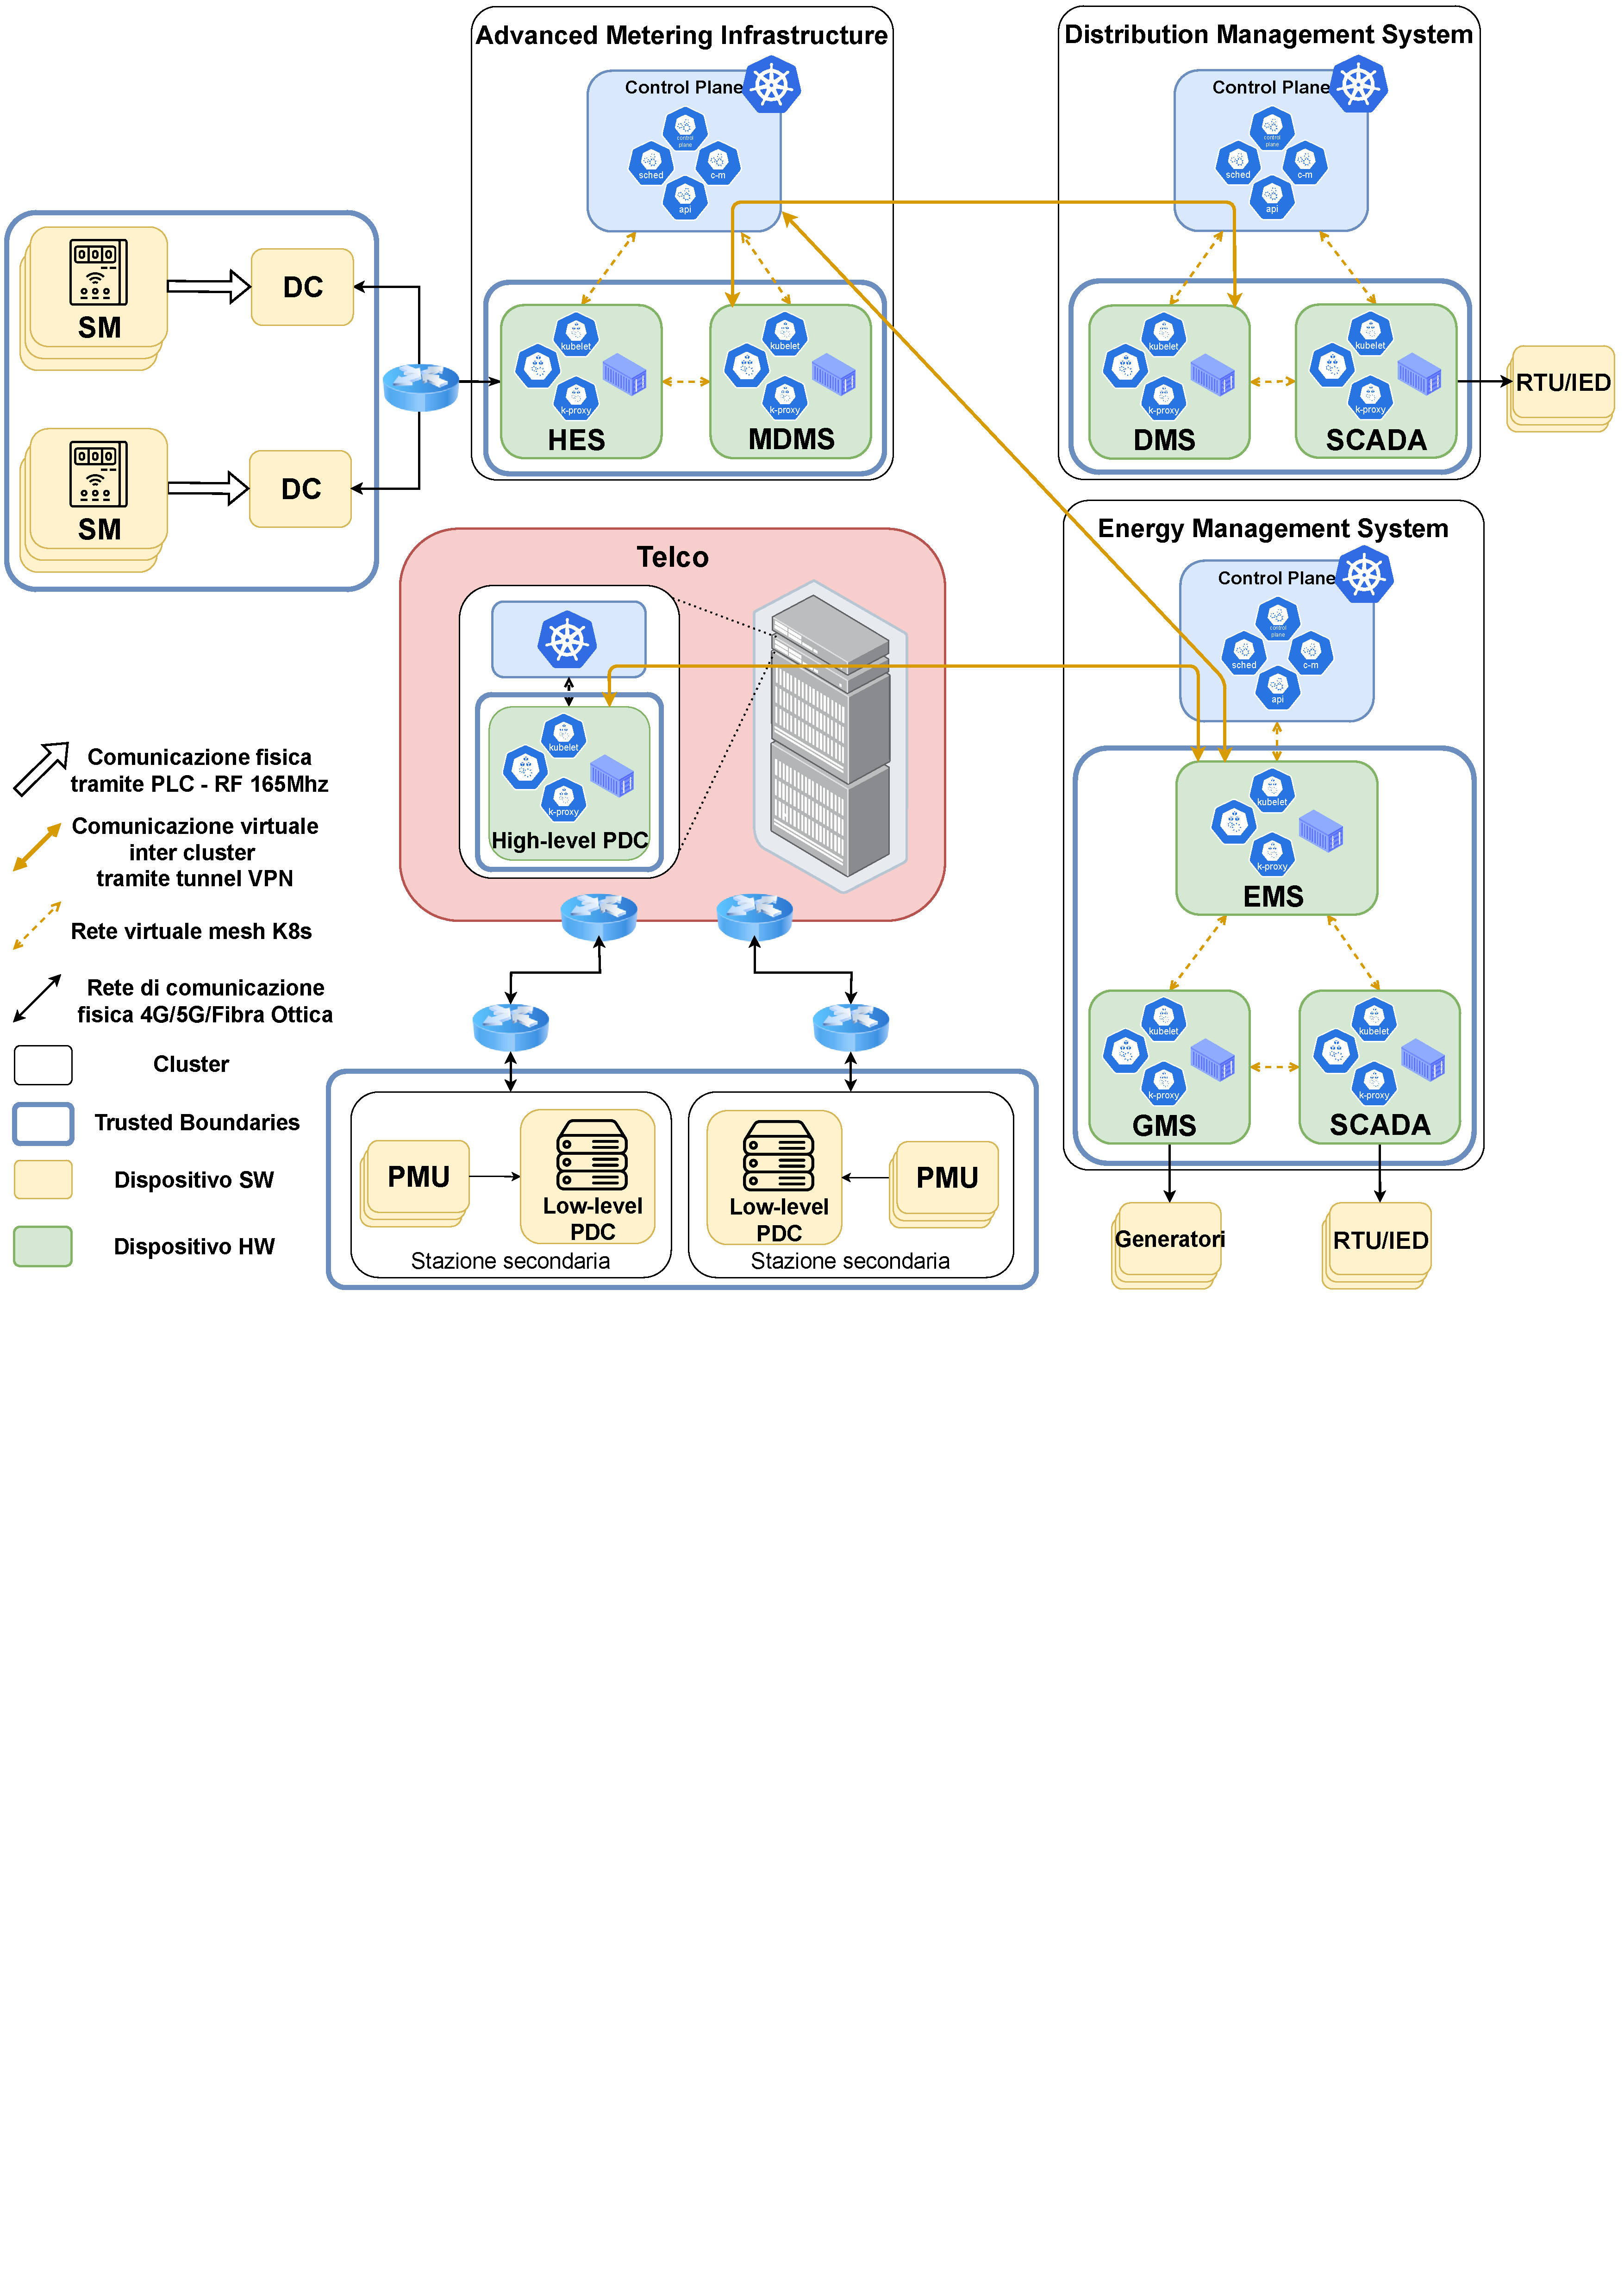
\includegraphics[trim= 0cm 36cm 0cm 0cm, clip, width=1\linewidth]{img/Cloud-native-Smart-Grid-v6.drawio.pdf}
    \caption{Architettura cloud native Smart Grid}
    \label{fig:arch-sm-cloud}
\end{figure}

\newpage
\subsection{Descrizione tecnica dei cluster Kubernetes}

% Ogni cluster Kubernetes (K8s) presente in Figura \ref{fig:arch-sm-cloud} è composto da due parti:

% \begin{itemize}
%     \item un Master contenente il control plane per la gestione dell'intero cluster, lo scheduler che gestisce la schedulazione delle risorse, le api fondamentali per l'accesso controllato delle risorse e dati dall'esterno e infine il ConfigMaps che memorizza i dati di configurazione.
%     \item una serie di \textit{Worker Node} contenenti la logica per il funzionamento e l'interfacciamento esterno dei servizi quali kublet e kublet-proxy (k-proxy) e il container run-time, software che permette l'esecuzione dei container\footnote{Rappresenta un'applicazione e tutte le sue dipendenze software. È eseguibili autonomamente.}. All'interno del worker node ci possono essere tanti pod\footnote{La più piccola unità di calcolo, servizio, che è possibile creare e gestire in Kubernetes.} il quale rappresenta un gruppo di uno o più container. Suddividere l'applicativo, ad esempio l'EMS, in tanti microservizi, permette di migliorare la sicurezza e accelerare la scalabilità anche a costo di una maggiore complessità.
% \end{itemize}

% All'interno di ogni cluster i vari nodi, chiamati \textit{pod}, riescono a comunicare con gli altri, comunicazione \textit{intra cluster pod-to-pod}, grazie alla rete mesh fornita dall'infrastruttura K8s. Questo permette lo scambio di dati constanti tra i vari nodi presenti nel cluster.


% La comunicazione esterna al cluster, inter cluster, è gestita dal Master K8s attraverso le API e, in questa possibile architettura, tramite un tunnel VPN (Virtual Private Network) per garantire i tre principi base della cybersecurity: Confidentiality, Integrity e Availability il cosiddetto \textit{CIA Triad} \cite{cia-triad}.


Come illustrato nel modello architetturale, ogni dominio funzionale è implementato come un cluster Kubernetes (K8s) autonomo. Un cluster K8s è composto da un insieme di macchine, chiamate nodi, che si dividono in due ruoli: nodi del \textit{Control Plane} e nodi \textit{Worker}.


\begin{enumerate}
    \item \textbf{Il \textit{Control Plane}}\\ Il \textit{Control Plane} è il cervello del cluster e ne gestisce lo stato globale. I suoi componenti principali, rappresentati schematicamente nella Figura \ref{fig:arch-sm-cloud}{}, sono:

    \begin{itemize}
        \item \textit{kube-apiserver}: Espone l'API di Kubernetes, fungendo da punto di ingresso per tutte le operazioni di gestione del cluster.
        \item \textit{etcd}: Un database chiave-valore consistente e ad alta disponibilità, utilizzato per memorizzare in modo persistente tutti i dati di configurazione e lo stato del cluster.
        \item \textit{kube-scheduler}: Assegna i nuovi Pod (le unità di esecuzione delle applicazioni) ai nodi \textit{Worker} disponibili, in base ai requisiti di risorse e alle policy definite.
        \item \textit{kube-controller-manager} (c-m): Esegue i controller che regolano lo stato del cluster, assicurando che lo stato attuale corrisponda a quello desiderato.
    \end{itemize}
    
    \item \textbf{\textit{Worker Nodes}}\\ I nodi \textit{Worker} sono le macchine (virtuali o fisiche) dove le applicazioni containerizzate vengono effettivamente eseguite. Ogni nodo \textit{Worker} esegue due agenti fondamentali:
    
    \begin{itemize}
        \item \textit{kubelet}: L'agente primario che comunica con il \textit{Control Plane} e si assicura che i container descritti nei Pod siano in esecuzione e in buono stato.
        \item \textit{kube-proxy}: Un proxy di rete che gestisce la comunicazione di rete sui singoli nodi, implementando le regole che permettono ai servizi di essere raggiungibili.
    \end{itemize}
\end{enumerate}



Le applicazioni, come ad esempio l'EMS, vengono scomposte in microservizi e impacchettate in uno o più container, che vengono poi eseguiti all'interno dei Pod. Questa architettura a microservizi, sebbene più complessa, offre vantaggi significativi in termini di scalabilità selettiva, resilienza e isolamento dei guasti.


\subsubsection{Comunicazione all'interno e tra i Cluster}

\begin{itemize}
    \item \textbf{Intra-Cluster:} All'interno di un singolo cluster, Kubernetes fornisce una rete virtuale flat (rete a mesh) che permette a tutti i Pod di comunicare direttamente tra loro, indipendentemente dal nodo su cui si trovano. Questo facilita lo scambio di dati ad alta velocità tra i microservizi che compongono un'applicazione.
    \item \textbf{Inter-Cluster:} La comunicazione tra cluster diversi e isolati (es. tra il cluster DMS e il cluster EMS) è un'operazione controllata e sicura. Viene gestita esponendo servizi specifici attraverso l'API server e, come proposto nel modello, incanalando il traffico attraverso un tunnel VPN (\textit{Virtual Private Network}). Questo approccio garantisce il rispetto della triade della sicurezza (Confidenzialità, Integrità, Disponibilità - \textit{CIA Triad}), proteggendo i dati scambiati tra i domini fidati \cite{cia-triad}.
\end{itemize}